\subsection{L'\OP, complémentaire de notre système\\ économique ?}

Serge Latouche, économiste français connu et reconnu, dit de notre société de consommation que la croissance économique est basée sur la publicité, le crédit et l'\op. La croissance serait un des moteurs de notre modèle économique, qui lui permettrait de continuer à exister et à avancer. Des liens existent entre la société de consommation dans laquelle nous vivons et l'\op. Celle-ci est particulièrement liée à la consommation et donc à la croissance. C'est en tout cas ce qu'il présente dans son livre \textit{Bon Pour la Casse}. Nous allons essayer d'expliciter son point de vue, qu'il décrit dans son essai.


\subsubsection{L'obsolescence et la consommation}
Dans notre modèle de société de consommation, le profit est au cœur de la vie d'une entreprise. En vendant suffisamment ses produits ou services, une société engrangera des bénéfices et pourra investir dans la bonne marche de son activité. Celle-ci pourra acheter de nouvelles machines, engager de nouveaux employés afin de s'agrandir, ce qui finalement lui permettra de se développer, et ainsi de suite. Cela lui permet par exemple de contrer plus facilement certains coups durs.

Bien entendu certaines entreprises vendent des produits qui se veulent de très bonne qualité, comme \textit{Lamborghini} ou \textit{Rolex}, et n'espèrent pas forcément un nombre de vente important, mais plutôt régulier, afin d'engranger tout de même des profits. Ainsi, la vente de l'un de leur produit ayant une forte valeur ajoutée leur permet de couvrir le faible taux de vente.

%\begin{figure}[h]
%\centerline{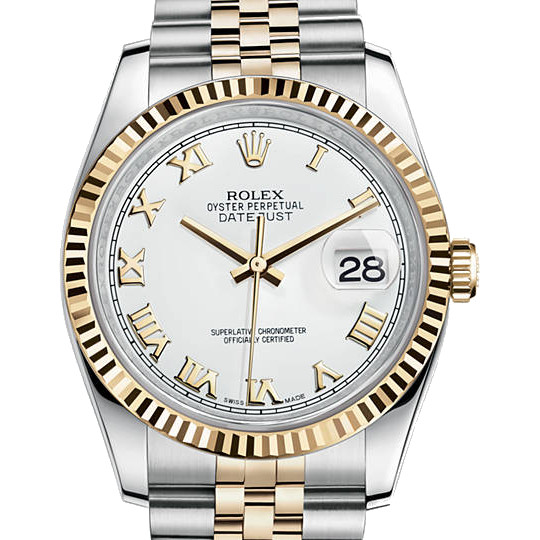
\includegraphics[scale=0.3]{Rsc/montre_rolex.jpg}}
%\caption{Les montres Rolex, un produit conçu pour durer. \textit{Source : www.rolex.com}}
%\label{Rolex}%attention, à placer après le caption, sinon référencera la section
%\end{figure}

\begin{wrapfigure}{l}{0.3\linewidth}
~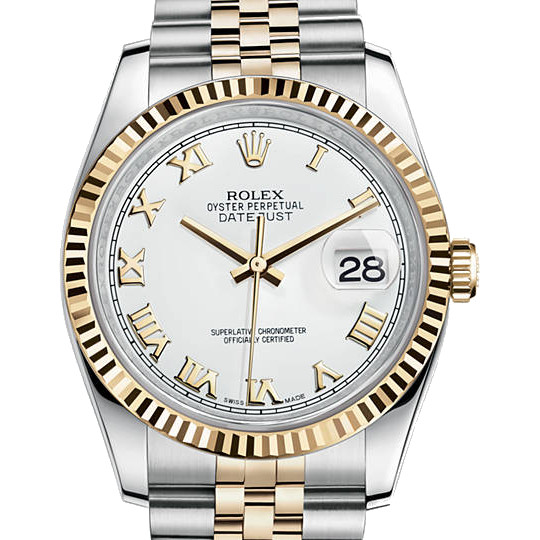
\includegraphics[scale=0.2]{Rsc/montre_rolex.jpg} 
\caption{Les montres Rolex, un produit conçu pour durer. \textit{Source : www.rolex.com}}
\label{Rolex}
\end{wrapfigure} 


\bigbreak
D'un autre coté, d'autres entreprises nécessitent de vendre en grande quantité afin d'amortir les coûts de production (ex : les charges fixes). Les revenus de l'entreprise sont donc fortement liées à la demande des consommateurs. Le but peut donc être pour une entreprise de pousser le consommateur à l'achat ou au rachat. Il existe plusieurs façons de faire :  le renouvellement des produits proposés, fidéliser les clients par la qualité des services ou des produits, attirer de nouveaux clients par la publicité, et bien d'autres. Ou encore par l'obsolescence programmée. Par l'incompatibilité logicielle ou par la technique. La publicité à outrance et uniquement dans le but de faire racheter aux clients des produits, peut également être considérée comme telle. Tout en sachant que l'\op technique n'est pas prouvée et nécessite de la retenue, comme expliqué par M. Clémentin (voir Annexe \ref{InterviewBClémentin}). Elle est en effet illégale en France suite à la loi sur les vices cachés.

Ainsi, en ce qui concerne l'\op psychologique, le produit courant est jeté au profit d'un nouveau. Il pourra être plus joli, comme présenté dans la dernière publicité vue à la télévision ou sur tout autre média, ou à la mode, grâce au marketing de la société, qui a réussi à en faire un produit connu que l'on veut acheter pour ne pas être "hors du coup". La publicité et le marketing en général sont devenus des secteurs importants dans les entreprises, du fait de leur forte influence sur le consommateur.

Si l'\op technique est avérée, cela signifie que nos produits sont prévus pour ne pas durer. Il suffit que le produit acheté soit particulièrement nécessaire, comme un réfrigérateur, ou très utile dans la vie de tout les jours, et il devient presque obligatoire d'en racheter un nouveau. Le pire est que l'on achète certains produits peu chers, puisque utile rarement ou de façon ponctuelle. Cela signifie souvent une moins bonne qualité. Mais on se dit qu'au prix où il a été acheté, on peut se permettre d'en acheter un neuf.

Dans le même temps, il est vrai que certaines entreprises ne permettent pas la réparation de leur produits. Plusieurs exemples existent, comme présentés dans le film \textit{Prêt à jeter} \cite{PretAjeter}. Certains portables sont impossibles à démonter, et quand bien même on tenterait de forcer nos appareils électroniques, le plus souvent de petites pièces qui permettaient à l'objet de tenir se cassent, rendant la réparation impossible. Pour des objets nécessitant des pièces détachées, celles-ci ne sont parfois plus disponibles à l'achat après une certaine période. Sauf que ces pièces détachées sont le plus souvent utilisées quelques années après l'achat, plutôt que dans l'année.

\bigbreak
Dans les années trente, des économistes proposaient de sortir de la crise en obligeant les consommateurs à jeter leur biens après une certaine date, afin d'en racheter de nouveaux, et ainsi relancer la consommation. Ce qui aurait permis selon eux de sortir de la crise. On retrouve ici l'idée d'une \op qui permet de contrebalancer la production de masse. 


\subsubsection{Le crédit, pour la consommation}
Lors de l'affaire du modèle de Détroit dans les années trente, qui opposaient \textit{General Motors} et \textit{Ford} (cf partie \ref{GM}), est apparue l'idée du crédit pour la consommation. La principe est triple. Pour les consommateurs, on a une façon de consommer d'un coup, et plus facilement, grâce à une importante somme d'argent remboursée sur la durée. Pour les banques, le crédit à la consommation est un formidable revenu. Et enfin, pour les entreprises vendant des produits cher (la voiture en est le meilleur exemple), cela permet à leur produit d'être acheté par la plupart des consommateur. Surtout des personnes ayant un faible revenu, qui n'auraient pu se payer des frais aussi importants.

Le système contient bien entendu des dérives, dont la plus connue est le surendettement, qui touche de nombreuses personnes. En 2013, en France, plus de deux cents mille dossiers de surendettement ont été déposés à la banque de France \cite{BanqueFranceEndettement}.


\subsubsection{La consommation, synonyme de croissance ?}
La consommation est souvent décrite comme premier moteur de la croissance. L'INSEE  décrit la croissance économique Française comme "l’évolution de la richesse produite sur le territoire français entre deux années ou entre deux trimestres. Cette richesse est appelée produit intérieur brut (PIB)" \cite{INSEEcroissance}.

Au cœur de ce PIB se trouve bien souvent les produits, fabriqués, achetés, et donc consommés. On a une croissance qui est ainsi particulièrement liée à l'envie d'achat. La consommation est donc bien l'un des moteur de la croissance, qui peu aussi compter sur les investissements des citoyens, des entreprises ou de l'état.

%\begin{figure}[h]
%\centerline{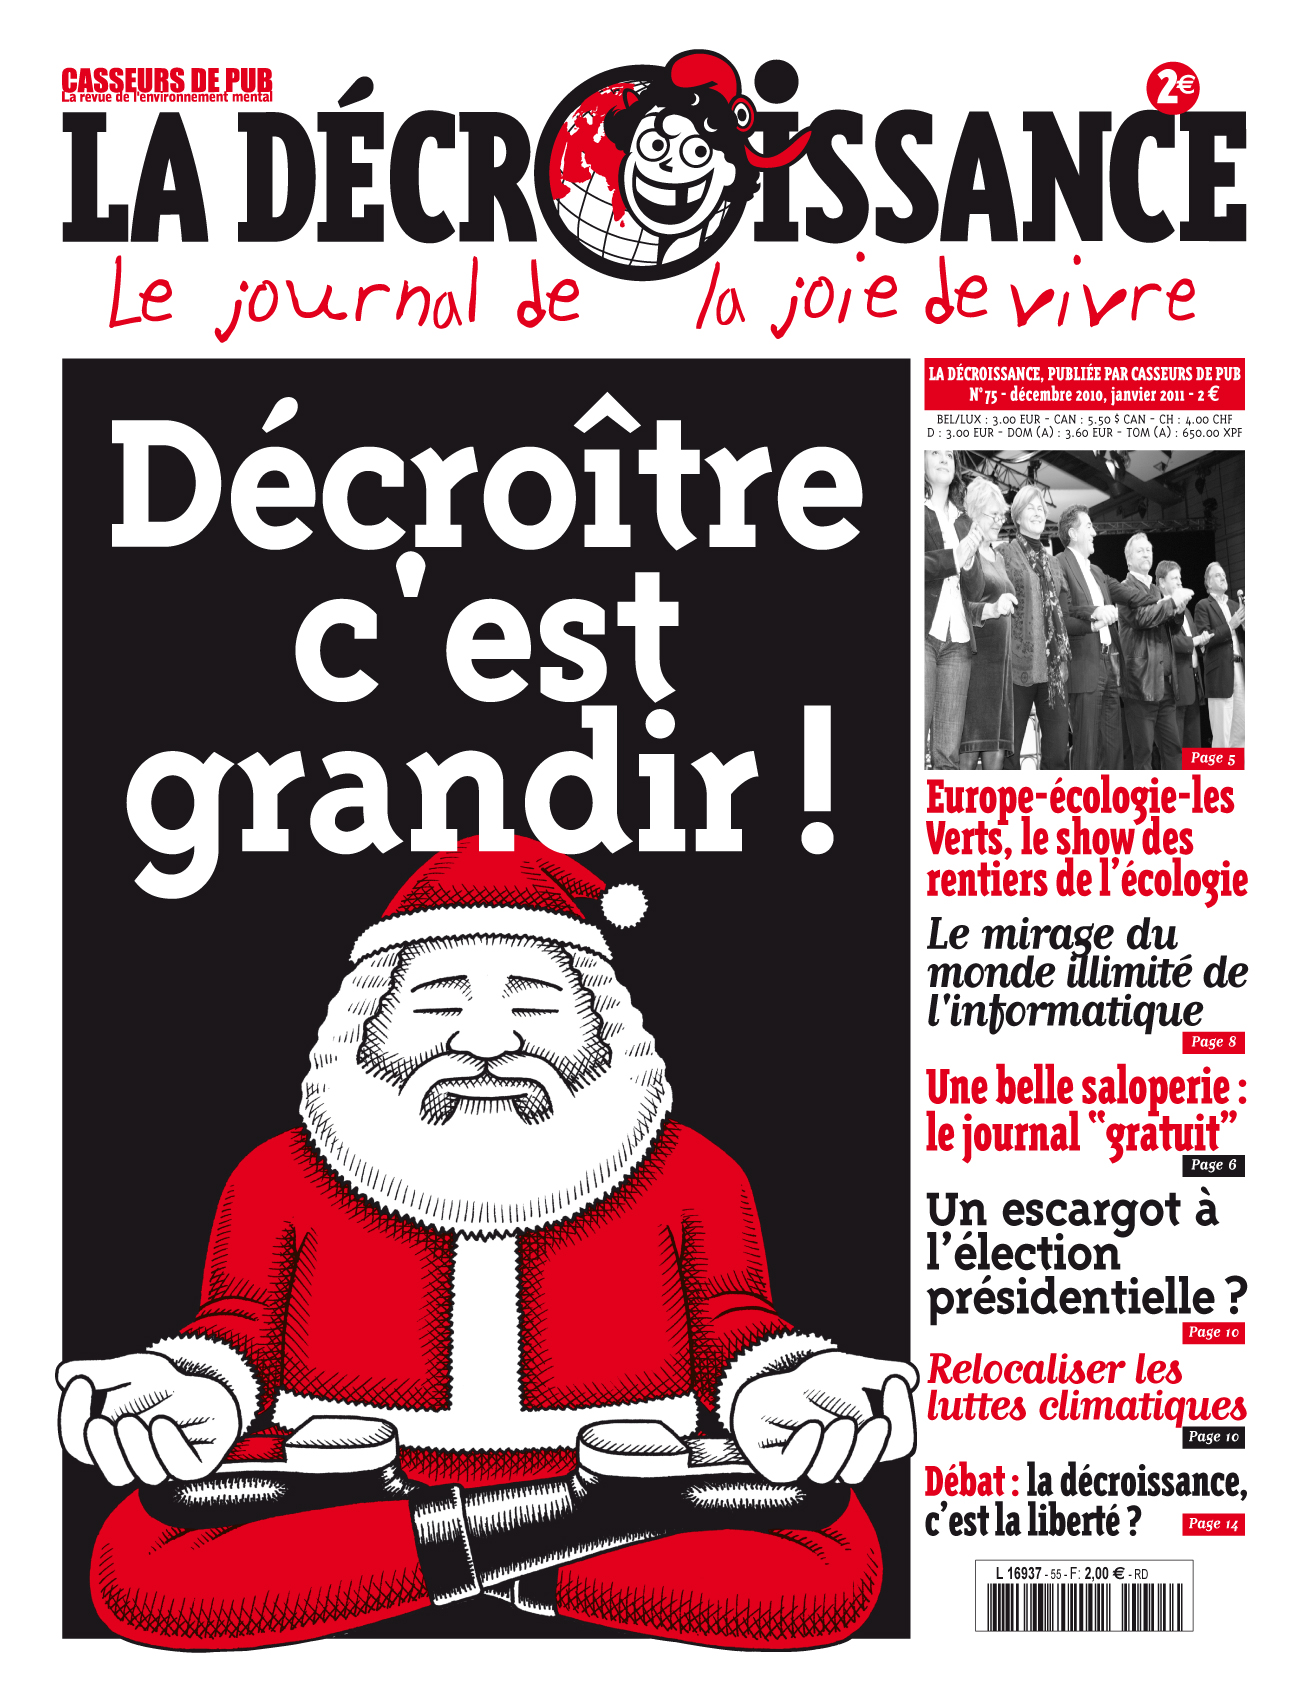
\includegraphics[scale=0.12]{Rsc/journal_La-Decroissance.jpg}}
%\caption{Le Journal La Décroissance, partisans de la lutte contre la consommation à outrance. \textit{Source : http://www.ladecroissance.net}}
%\label{Rolex}%attention, à placer après le caption, sinon référencera la section
%\end{figure}

\begin{wrapfigure}{l}{0.3\linewidth}
~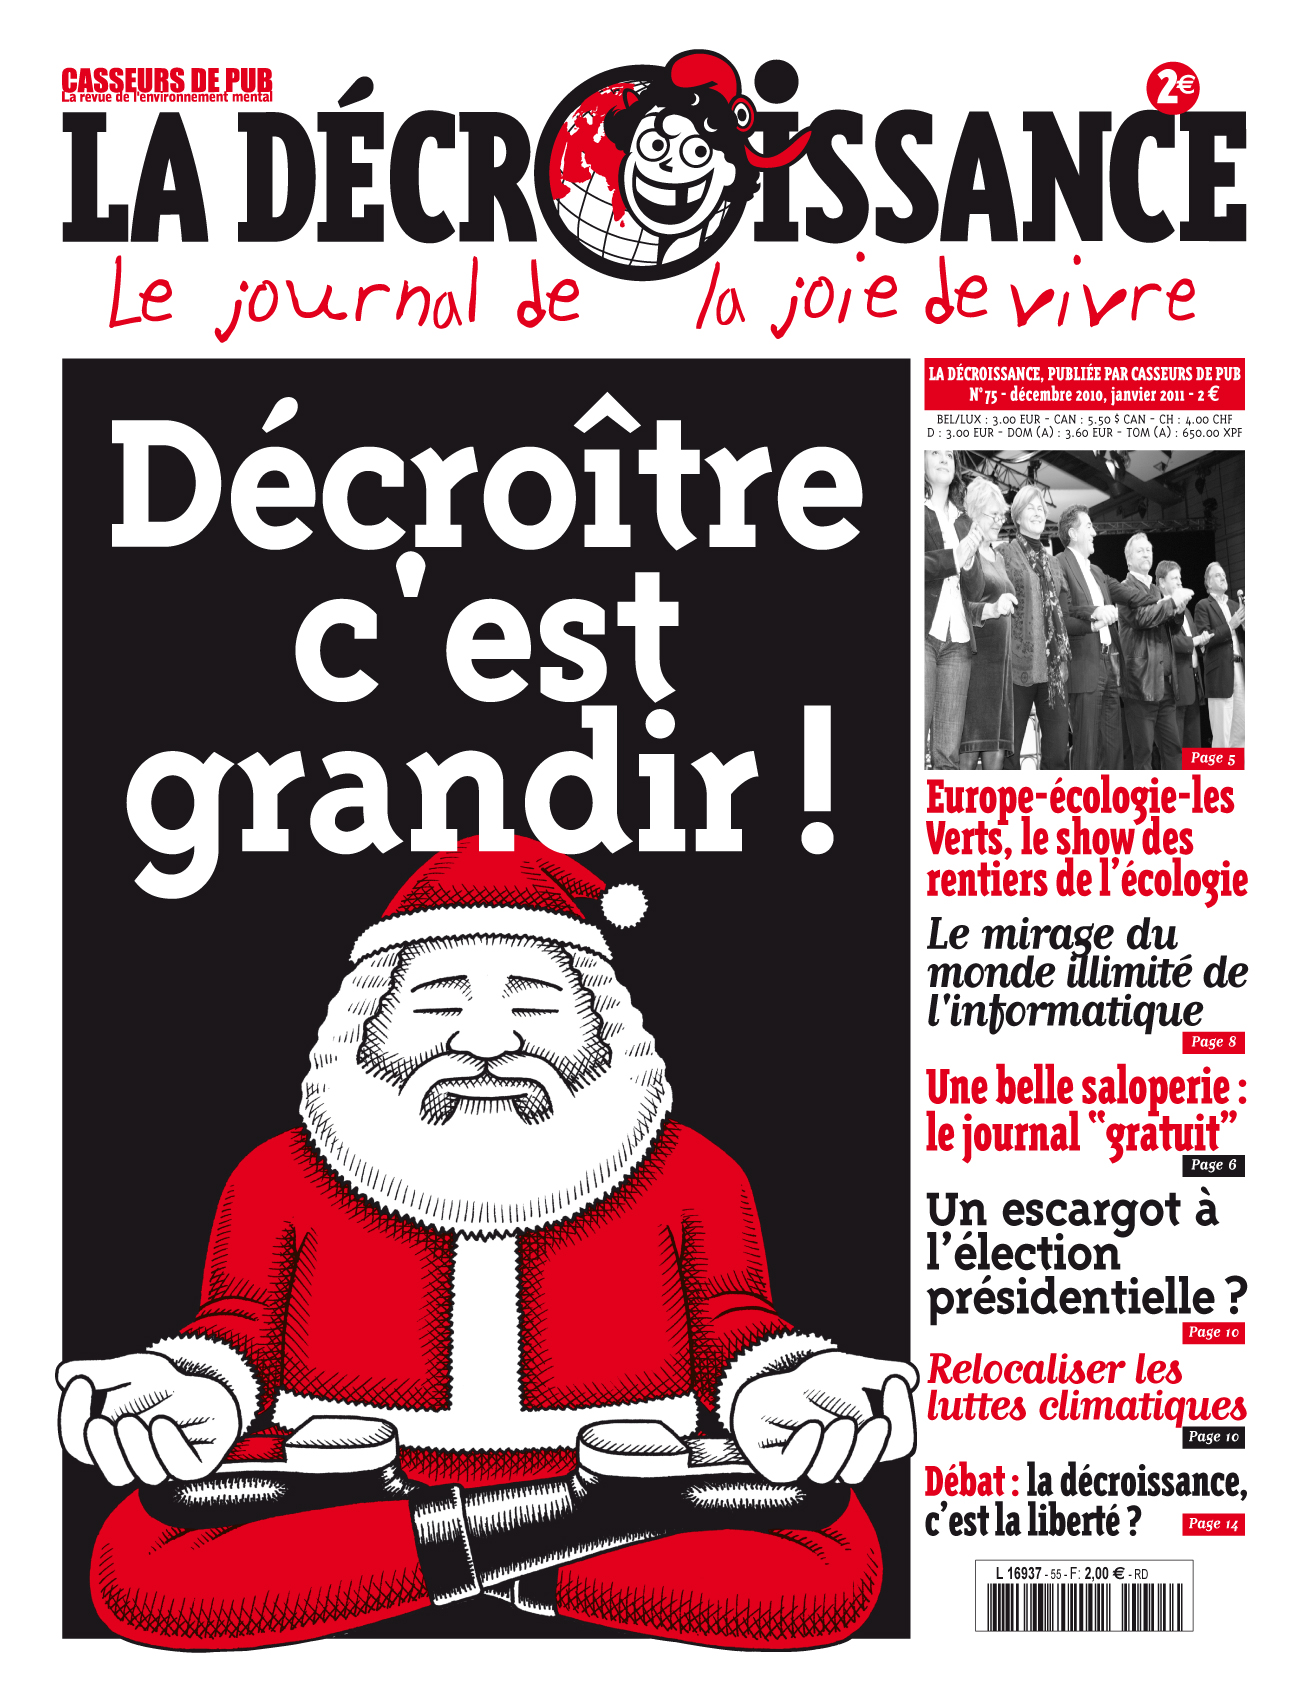
\includegraphics[scale=0.1]{Rsc/journal_La-Decroissance.jpg} 
\caption{Le Journal La Décroissance, partisans de la lutte contre la consommation à outrance. \textit{Source : http://www.ladecroissance.net}}
\label{journalDecroissance}
\end{wrapfigure} 


\bigbreak
Des économistes ou politiques affirment que nous devons avoir une croissance la plus forte possible, tandis que d'autres pointent du doigt les dérives de la croissance. Pollutions, épuisement des ressources ou augmentation des inégalités sociales sont autant de problèmes provoqués par la croissance. Ainsi certains altermondialistes, journalistes ou penseurs proposent de sortir de ce système et d'adopter la notion de Décroissance. Il s'agit d'un terme qui peut faire peur, mais cela signifie principalement la modération ou l'arrêt de la surconsommation, ainsi que la réflexion sur une autre société.





%CREDITS !!!!!!!!!!!!!!!!!!!!!!!!!!!!!!!!!!!
%consommation --> emplois !
%publicité --> emplois !
%de plus en plus de croissance --> on veut toujours plus --> toujours plus de gens à rechercher profits --> plus de production --> OP




%\subsection{Obsolescence et consommation}
%
%Dans notre modèle de société de consommation, le profit est au cœur de la vie d'une entreprise. En vendant suffisamment ses produits ou services, une société engrangera des bénéfices et pourra investir dans la bonne marche de son activité. Celle-ci pourra acheter de nouvelles machines, engager de nouveaux employés afin de s'agrandir, ce qui finalement lui permettra de s'agrandir, et ainsi de suite.
%
%% Pour cela, il lui faut donc réussir à écouler ses stocks, afin de vendre le plus possible, et donc susciter la consommation. Cela se fait souvent au travers du marketing et plus particulièrement de la publicité, qui nous incite à acheter le produit d'une marque X. L'idée est que certains produits ou marques nouvelles sur le marché doivent être connus du grand public, sans quoi celui-ci risque de ne pas vouloir du produit.
%
%\bigbreak
%% Cependant, si le produit acheté est durable, du fait de sa bonne qualité ou de l'inutilité de son rachat, l'entreprise ne gagnera qu'une seule fois par acheteur, et finit par ne plus avoir de clients.
%%Il faut donc de nouveau pousser le consommateur à l'achat par la publicité, le renouvellement des produits proposés, ou par l'obsolescence programmée. 
%Ainsi, le produit courant est jeté au profit d'un nouveau. Il pourra être plus joli ou à la mode, comme présenté dans la dernière publicité vue à la télévision ou sur tout autre média, ou bien le produit ne sera  tout simplement plus fonctionnel. Bien entendu certaines entreprises vendent des produits qui se veulent de très bonne qualité réussissent à tirer leur épingle du jeu et à  
%
%%La dernière raison peut être totalement involontaire, 
%alors le produit devra être racheté si le consommateur en a l'utilité. Inversement, le dysfonctionnement serait prévu et recherché par le fabricant. Ici apparaît le concept de l'obsolescence programmée : le produit est prévu dans sa construction pour ne durer qu'un certain temps, comme une année par exemple. Au bout de cette période, le consommateur serait donc poussé au rachat s'il souhaite continuer à bénéficier de l'avantage procuré par le produit.
%
%Tout cela reste une hypothèse, étant donné que seuls quelques exemples d'\op avérée ont filtré. Cela ne signifie pas qu'elle n'existe pas. Simplement, comme le disait M. Clémentin (----ref interview----), on ne peut affirmer qu'elle existe.
%
%\bigbreak
%Dans le même temps, il est vrai que certaines entreprises ne permettent pas la réparation de leur produits. Plusieurs exemples existent, comme présentés dans le film \textit{Prêt à jeter} \cite{PretAjeter}. Certains portables sont impossibles à démonter, et quand bien même on tenterait de forcer nos appareils électroniques, le plus souvent de petites pièces qui permettaient à l'objet de tenir se cassent, rendant la réparation impossible. Pour des objets nécessitant des pièces détachées, celles-ci ne sont parfois plus disponibles à l'achat après une certaine période. Sauf que ces pièces détachées sont le plus souvent utilisées quelques années après l'achat, plutôt que dans l'année.
%
%Dans les années trente, des économistes proposaient de sortir de la crise en obligeant les consommateurs à jeter leur biens après une certaine date, afin d'en racheter de nouveaux, et ainsi relancer la consommation. Ce qui aurait permis selon eux de sortir de la crise. On retrouve ici l'idée d'une \op qui permet de contrebalancer la production de masse.
%

